\documentclass[11pt,a4paper]{article}

\usepackage[utf8]{inputenc}
\usepackage[T1]{fontenc}
\usepackage[margin=2.5cm]{geometry}
\usepackage{xcolor}
\usepackage{titlesec}
\usepackage{enumitem}
\usepackage{hyperref}
\usepackage{graphicx}
\usepackage{booktabs}
\usepackage{array}
\usepackage{fancyhdr}
\usepackage{parskip}

\definecolor{teal}{HTML}{1A5276}
\definecolor{accent}{HTML}{2E86C1}
\definecolor{dark}{HTML}{1C2833}
\definecolor{gray}{HTML}{7F8C8D}

\hypersetup{colorlinks=true, urlcolor=accent, linkcolor=teal}

\titleformat{\section}{\color{teal}\Large\bfseries}{\thesection}{0.6em}{}
\titleformat{\subsection}{\color{teal}\large\bfseries}{\thesubsection}{0.6em}{}

\pagestyle{fancy}
\fancyhf{}
\fancyhead[L]{\small\color{gray} Prédiction du churn client — Rapport de projet}
\fancyhead[R]{\small\color{gray}\thepage}
\renewcommand{\headrulewidth}{0.4pt}

\newcommand{\keyfact}[1]{%
  \begin{center}
  \colorbox{blue!8}{\parbox{0.92\linewidth}{\vspace{4pt}#1\vspace{4pt}}}
  \end{center}
}

\begin{document}

\begin{titlepage}
\centering
\vspace*{2cm}
{\Huge\bfseries\color{teal} Prédiction du Churn Client}\\[8pt]
{\Large\color{dark} Un projet de Machine Learning supervisé de bout en bout}\\[40pt]

{\large André Kevin LOUKANOU LOUZOLO}\\[4pt]
{\color{gray} Master Mathématiques Appliquées — Statistiques et Data Science}\\
{\color{gray} Université d'Aix-Marseille}\\[40pt]

\vspace{2cm}
{\color{dark}\textit{Projet réalisé sur le jeu de données public IBM Telco Customer Churn\\
(7~043 clients), pour démontrer le cycle complet d'un projet de classification supervisée.}}

\vfill
{\small\color{gray} \today}
\end{titlepage}

\tableofcontents
\newpage

% ════════════════════════════════════════════
\section{Contexte et cadrage du problème}
% ════════════════════════════════════════════

Le \textbf{churn} (attrition) désigne la perte de clients par une entreprise. L'objectif est de construire un modèle de \textit{machine learning} supervisé capable d'identifier, en amont, les clients les plus susceptibles de résilier — afin de permettre une action de rétention ciblée avant le départ effectif.

\subsection{Jeu de données}
Ce projet utilise le jeu de données public \textbf{IBM Telco Customer Churn} (7~043 clients, 21 variables), un des jeux de données de référence en Data Science pour ce type de problème.

\subsection{Pourquoi l'accuracy seule ne suffit pas}
Le churn est déséquilibré par nature : \textbf{26,5\,\%} des clients de ce jeu de données sont partis, contre 73,5\,\% restés. Un modèle prédisant systématiquement \og le client reste \fg{} obtiendrait déjà 73,5\,\% d'accuracy sans détecter le moindre départ. Le choix des métriques (precision, recall, F1) est donc traité comme un enjeu central, et la priorité métier retenue est de \textbf{maximiser le recall} : le coût d'un client perdu est jugé supérieur au coût d'une relance inutile.

% ════════════════════════════════════════════
\section{Données et qualité}
% ════════════════════════════════════════════

Le jeu de données comprend des variables démographiques (genre, âge, situation familiale), contractuelles (type de contrat, mode de paiement), d'usage (ancienneté, services souscrits) et financières (charges mensuelles et totales).

\subsection{Un défaut de qualité de données réel}
La colonne \texttt{TotalCharges}, censée être numérique, est stockée en texte et contient \textbf{11 valeurs \guillemotleft~vides déguisées\guillemotright{}} (une chaîne composée uniquement d'un espace) plutôt que de vraies valeurs manquantes (\texttt{NaN}) — ces 11 clients ont tous une ancienneté (\texttt{tenure}) de 0 mois : ils n'ont simplement pas encore reçu de première facture totale. Ce défaut est invisible à un simple \texttt{isnull()} et nécessite une vérification plus fine (type de colonne, recherche de chaînes vides) pour être détecté.

Ces 11 lignes (0,16\,\% du jeu de données) ont été retirées après conversion explicite en type numérique.

% ════════════════════════════════════════════
\section{Analyse exploratoire (EDA)}
% ════════════════════════════════════════════

\begin{figure}[h]
\centering
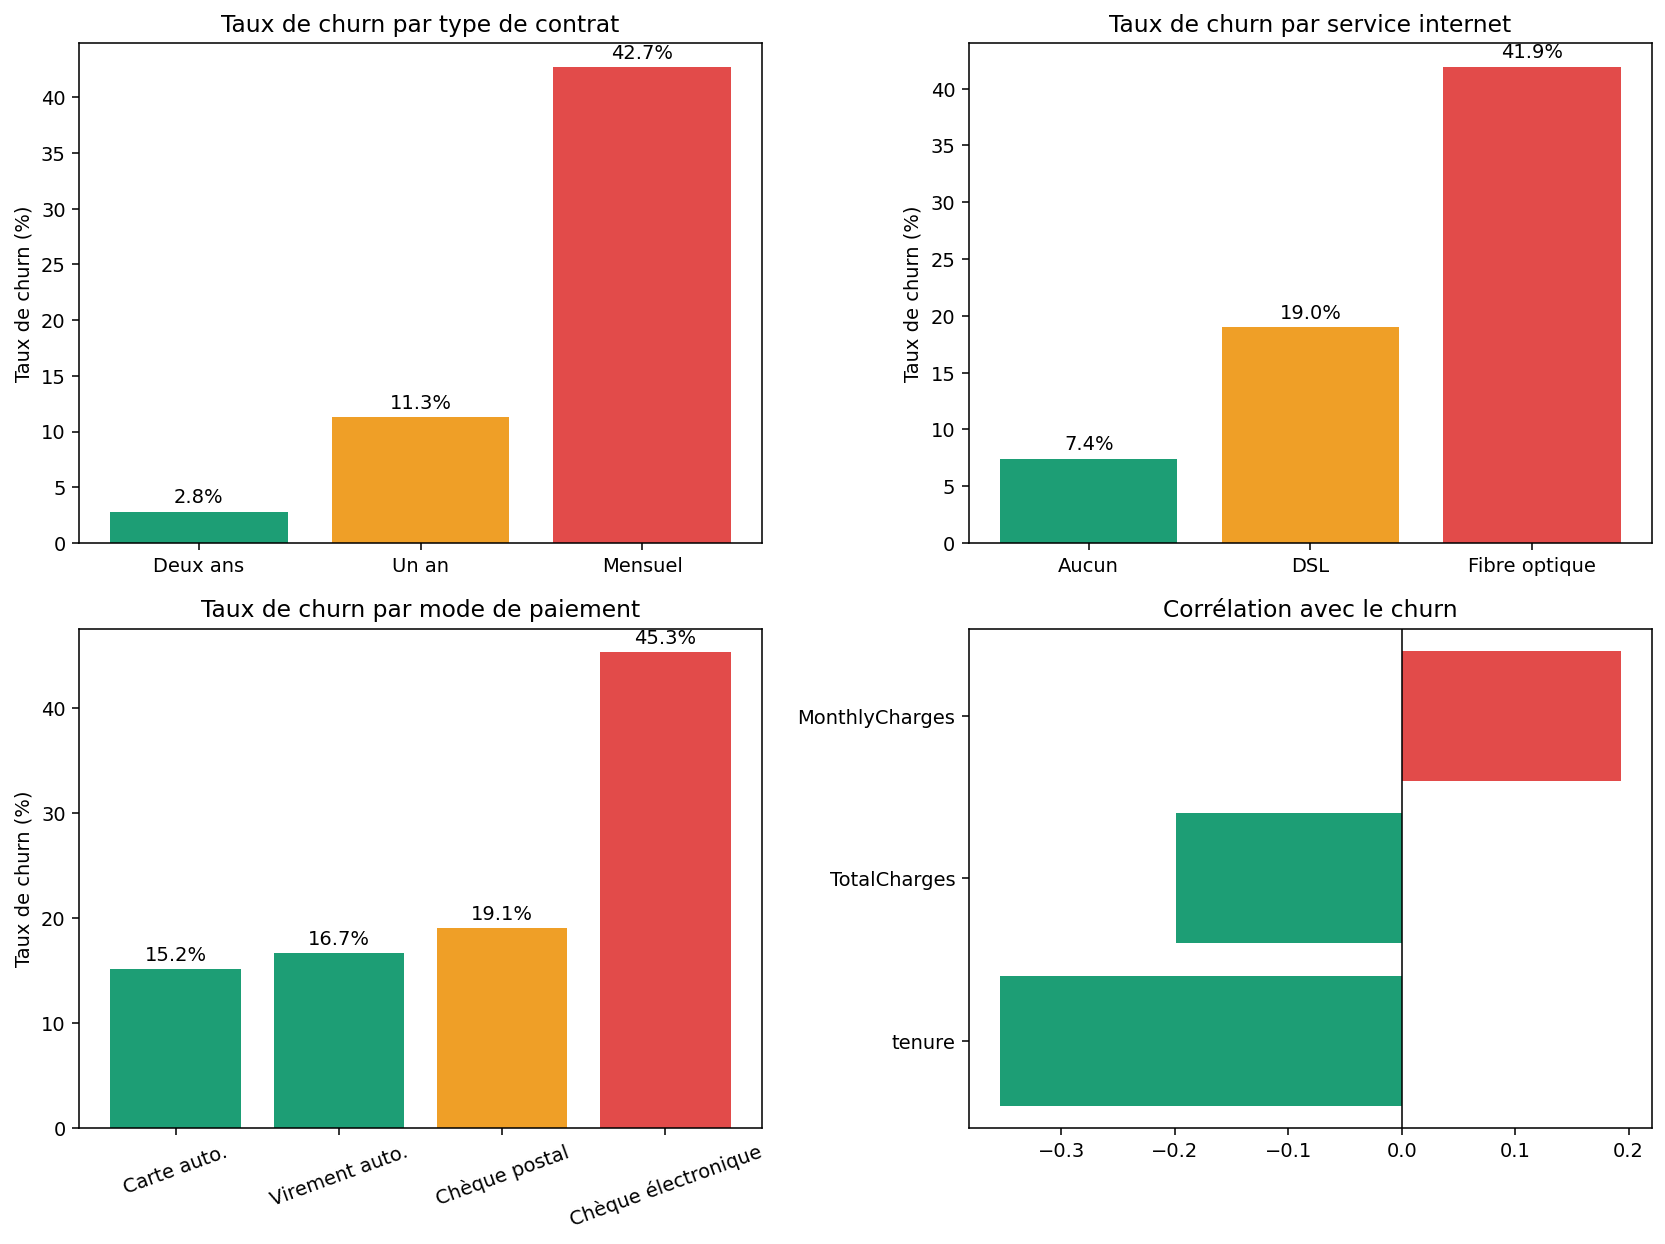
\includegraphics[width=0.95\linewidth]{figures/eda_overview.png}
\caption{Taux de churn par type de contrat, service internet, mode de paiement, et corrélations des variables numériques avec le churn.}
\end{figure}

\subsection{Principaux signaux identifiés}
\begin{itemize}
\item \textbf{Type de contrat} : \textbf{42,7\,\%} de churn en contrat mensuel, contre seulement \textbf{2,8\,\%} en engagement deux ans — un facteur de risque 15 fois plus élevé.
\item \textbf{Mode de paiement} : le chèque électronique est associé à \textbf{45,3\,\%} de churn, contre 15 à 19\,\% pour les autres modes — les modes de paiement automatisés apparaissent nettement protecteurs.
\item \textbf{Service internet} : la fibre optique atteint \textbf{41,9\,\%} de churn, contre 19\,\% en ADSL — un signal contre-intuitif (meilleur service, plus de départs), généralement attribué à un effet prix/concurrence.
\item \textbf{Ancienneté (\texttt{tenure})} : corrélation négative la plus forte parmi les variables numériques ($r=-0{,}354$).
\item \textbf{Redondance détectée} : \texttt{tenure} et \texttt{TotalCharges} sont fortement corrélées ($r=0{,}826$), un point traité lors de la préparation des données.
\end{itemize}

% ════════════════════════════════════════════
\section{Préparation des données}
% ════════════════════════════════════════════

\begin{enumerate}[label=\arabic*.]
\item Suppression de l'identifiant client et conversion de la variable cible en binaire.
\item Création d'une variable dérivée \texttt{charge\_moyenne\_reelle} = \texttt{TotalCharges} / \texttt{tenure}, pour limiter la redondance entre les deux variables sans en supprimer aucune.
\item Encodage binaire simple pour les variables à 2 modalités (Oui/Non, genre), et one-hot encoding (\texttt{drop\_first=True}) pour les variables à 3 modalités ou plus (type de contrat, service internet, options souscrites, mode de paiement).
\item Standardisation des variables numériques.
\item Séparation entraînement/test (80/20), stratifiée pour préserver le taux de churn (26,6\,\%) dans les deux ensembles.
\end{enumerate}

\keyfact{\textbf{Point de vigilance identifié :} plusieurs variables d'options (sécurité en ligne, support technique, streaming...) partagent une modalité \og No internet service \fg{}, strictement redondante avec \texttt{InternetService = No}. Un client sans internet ne peut logiquement pas avoir ces services — ces colonnes encodées portent donc en partie la même information.}

% ════════════════════════════════════════════
\section{Modélisation et comparaison}
% ════════════════════════════════════════════

Trois modèles ont été comparés par validation croisée à 5 plis :

\begin{center}
\begin{tabular}{lcc}
\toprule
\textbf{Modèle} & \textbf{Recall moyen (5-fold)} & \textbf{Stabilité} \\
\midrule
\textbf{Régression logistique} & \textbf{0,805} & $\pm$0,022 \\
Random Forest & 0,477 & $\pm$0,018 \\
Gradient Boosting & 0,523 & $\pm$0,023 \\
\bottomrule
\end{tabular}
\end{center}

La régression logistique domine nettement, un résultat cohérent avec un projet préliminaire mené sur un jeu de données simulé — la conclusion se vérifie donc sur deux jeux de données distincts, ce qui renforce sa robustesse.

\begin{figure}[h]
\centering
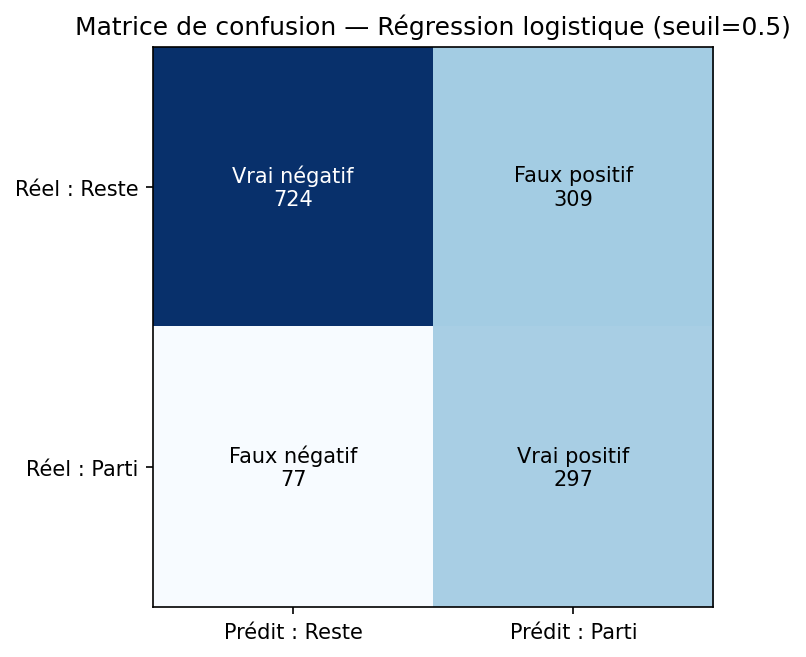
\includegraphics[width=0.55\linewidth]{figures/confusion_matrix.png}
\caption{Matrice de confusion du modèle retenu (régression logistique, seuil = 0,5) sur le jeu de test (1~407 clients).}
\end{figure}

% ════════════════════════════════════════════
\section{Évaluation détaillée}
% ════════════════════════════════════════════

\begin{center}
\begin{tabular}{lccc}
\toprule
\textbf{Classe} & \textbf{Precision} & \textbf{Recall} & \textbf{F1-score} \\
\midrule
Reste (0) & 0,90 & 0,70 & 0,79 \\
\textbf{Parti (1)} & \textbf{0,49} & \textbf{0,79} & \textbf{0,61} \\
\midrule
Accuracy globale & \multicolumn{3}{c}{0,73} \\
\bottomrule
\end{tabular}
\end{center}

\textbf{Lecture métier :} sur 374 clients réellement partis dans le jeu de test, le modèle en détecte \textbf{297 (79\,\%)}, au prix de 309 fausses alertes sur 1~033 clients réellement restés.

\subsection{Sur le choix du seuil de décision}
Une analyse de la courbe precision/recall a identifié un seuil de 0,61 comme optimal au sens du F1-score (F1 = 0,627, contre $\sim$0,60 au seuil par défaut). Ce seuil a été \textbf{délibérément écarté} : il ferait chuter le recall de 0,79 à environ 0,60, contraire à la priorité métier définie au cadrage (maximiser la détection des départs). Le seuil par défaut (0,5) est conservé.

% ════════════════════════════════════════════
\section{Interprétation du modèle}
% ════════════════════════════════════════════

\begin{figure}[h]
\centering
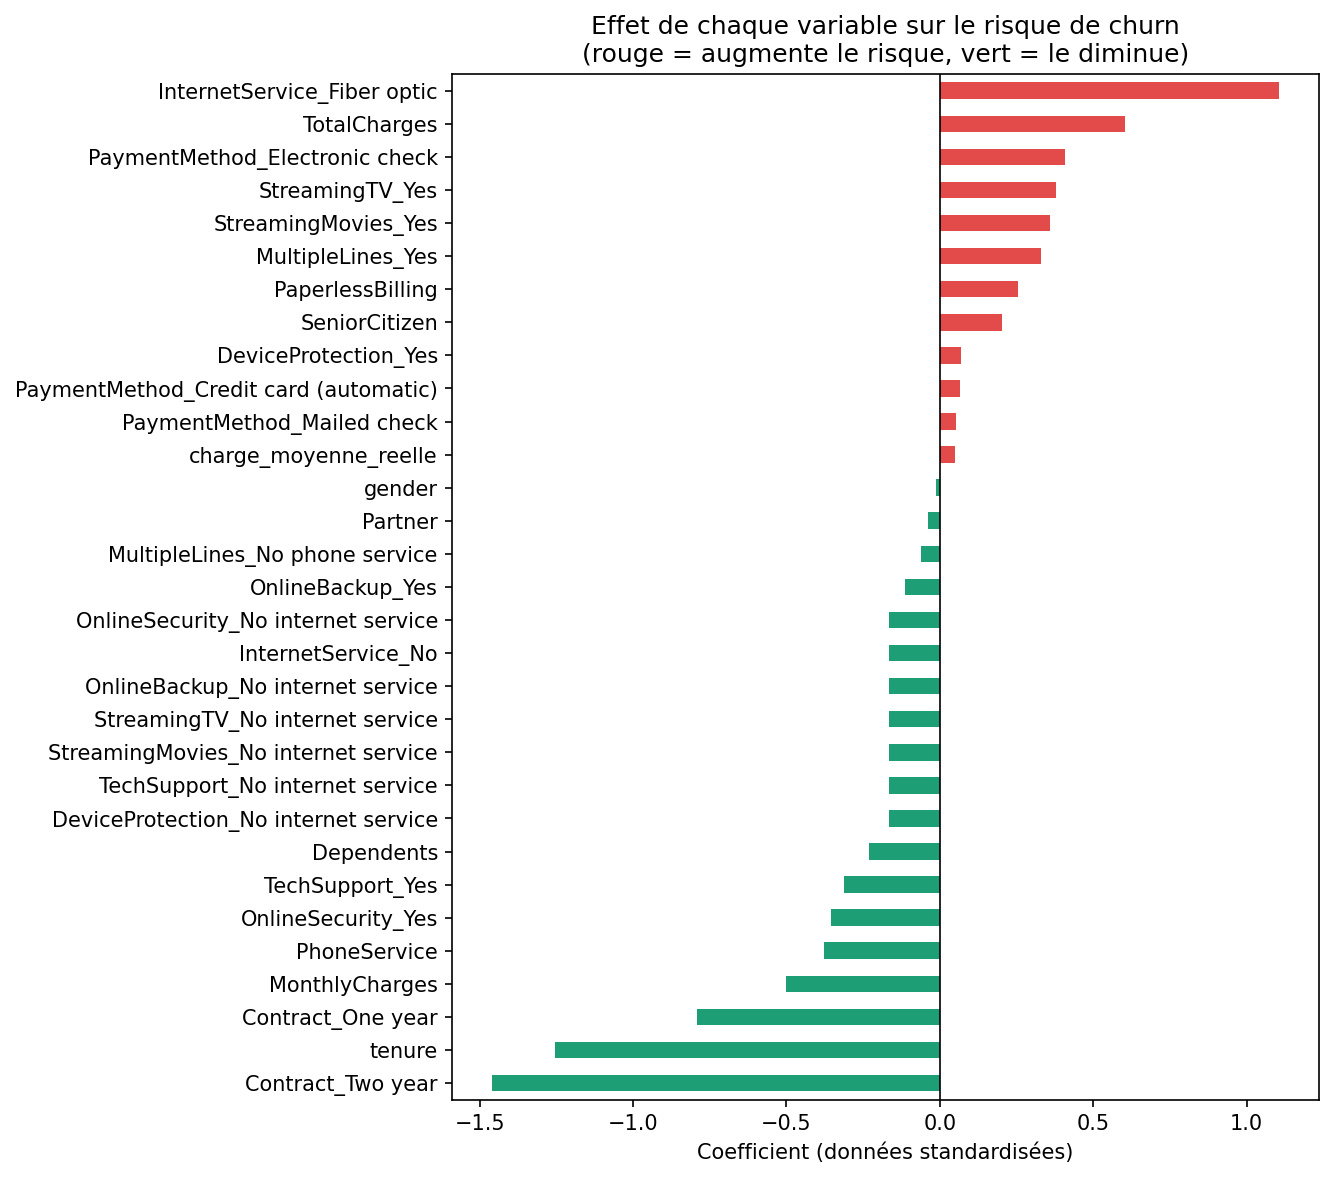
\includegraphics[width=0.85\linewidth]{figures/coefficients_plot.png}
\caption{Coefficients de la régression logistique (données standardisées).}
\end{figure}

\subsection{Facteurs qui augmentent le risque de départ}
\begin{enumerate}[label=\arabic*.]
\item \textbf{Service internet fibre optique} — le facteur de risque le plus fort de tout le modèle
\item \textbf{Paiement par chèque électronique}
\item \textbf{Options de streaming souscrites (TV, films)}
\end{enumerate}

\subsection{Facteurs qui protègent contre le départ}
\begin{enumerate}[label=\arabic*.]
\item \textbf{Contrat de deux ans} — le facteur protecteur le plus fort
\item \textbf{Ancienneté (\texttt{tenure})}
\item \textbf{Contrat d'un an}
\item \textbf{Support technique et sécurité en ligne souscrits}
\end{enumerate}

\subsection{Un point de rigueur méthodologique}
Le coefficient de \texttt{TotalCharges} est positif (+0,604) dans le modèle final malgré une corrélation brute négative en exploration ($r=-0{,}199$). Ce changement de signe s'explique par la forte redondance avec \texttt{tenure} : une fois l'effet de l'ancienneté isolé, le signal résiduel de \texttt{TotalCharges} et \texttt{MonthlyCharges} devient difficile à interpréter isolément. \textbf{Ces trois variables corrélées doivent être lues comme un ensemble, non individuellement.}

% ════════════════════════════════════════════
\section{Recommandation business}
% ════════════════════════════════════════════

\keyfact{\textbf{Profil du client à risque prioritaire :} client en contrat mensuel, équipé de la fibre optique, payant par chèque électronique, avec une faible ancienneté et sans options de protection souscrites (sécurité en ligne, support technique).}

\textbf{Actions recommandées, par ordre de priorité :}
\begin{enumerate}[label=\arabic*.]
\item \textbf{Inciter au passage vers un contrat engagé} (remise, mois offerts) dès les premiers mois, en priorité pour les clients fibre.
\item \textbf{Investiguer la satisfaction des clients fibre} : le prix plus élevé et/ou la qualité perçue du service semblent être des facteurs de churn directs.
\item \textbf{Encourager le passage à un prélèvement automatique} pour les clients payant par chèque électronique, un mode de paiement fortement associé au désengagement.
\end{enumerate}

Le modèle détecte 79\,\% des départs réels, un compromis jugé raisonnable pour déclencher des actions de rétention à faible coût plutôt qu'une décision coûteuse et irréversible.

\subsection{Limites}
\begin{itemize}
\item Les coefficients de \texttt{tenure}, \texttt{MonthlyCharges} et \texttt{TotalCharges} doivent être interprétés conjointement, en raison de leur forte corrélation mutuelle.
\item Le seuil de décision (0,5) reflète une priorité métier assumée (maximiser le recall) ; un contexte d'entreprise différent, avec un coût de fausse alerte plus élevé, justifierait un seuil plus restrictif.
\end{itemize}

\vspace{20pt}
\begin{center}
\textit{Stack technique : Python, Pandas, Scikit-learn, Matplotlib}\\
\textit{Jeu de données : IBM Telco Customer Churn (domaine public)}
\end{center}

\end{document}
